\documentclass[a4paper,12pt]{article}
\usepackage[]{inputenc}
\usepackage[russian]{babel}
\usepackage[left=30mm, top=20mm, right=10mm, bottom=20mm, nohead, nofoot]{geometry}
\usepackage{indentfirst}
\usepackage{listings}


\title{Файловая организация базовых программных средств в робототехнических платформах}
\author{github:ArtemZaZ}
\date{Январь 2020}

\usepackage{natbib}
\usepackage{graphicx}

\begin{document}
\renewcommand{\baselinestretch}{1.5}
\setlength{\parindent}{5ex}

\maketitle

\begin{center}
Version 0.1b
\end{center}

\section{Введение}
С увеличением возможностей робототехнических платформ, а также их разнообразия в нашем отделе, увеличивается объем и сложность программных частей и модулей, необходимых для их эксплуатации. Одной из проблем, возникающих в результате этого, является отсутствие организации самих программных средств.     

\section{Edubot}
В качестве примера и описания дальнейших концепций будем рассматривать робототехническую платформу Edubot (рисунок 1).

\begin{figure}[h!]
\centering
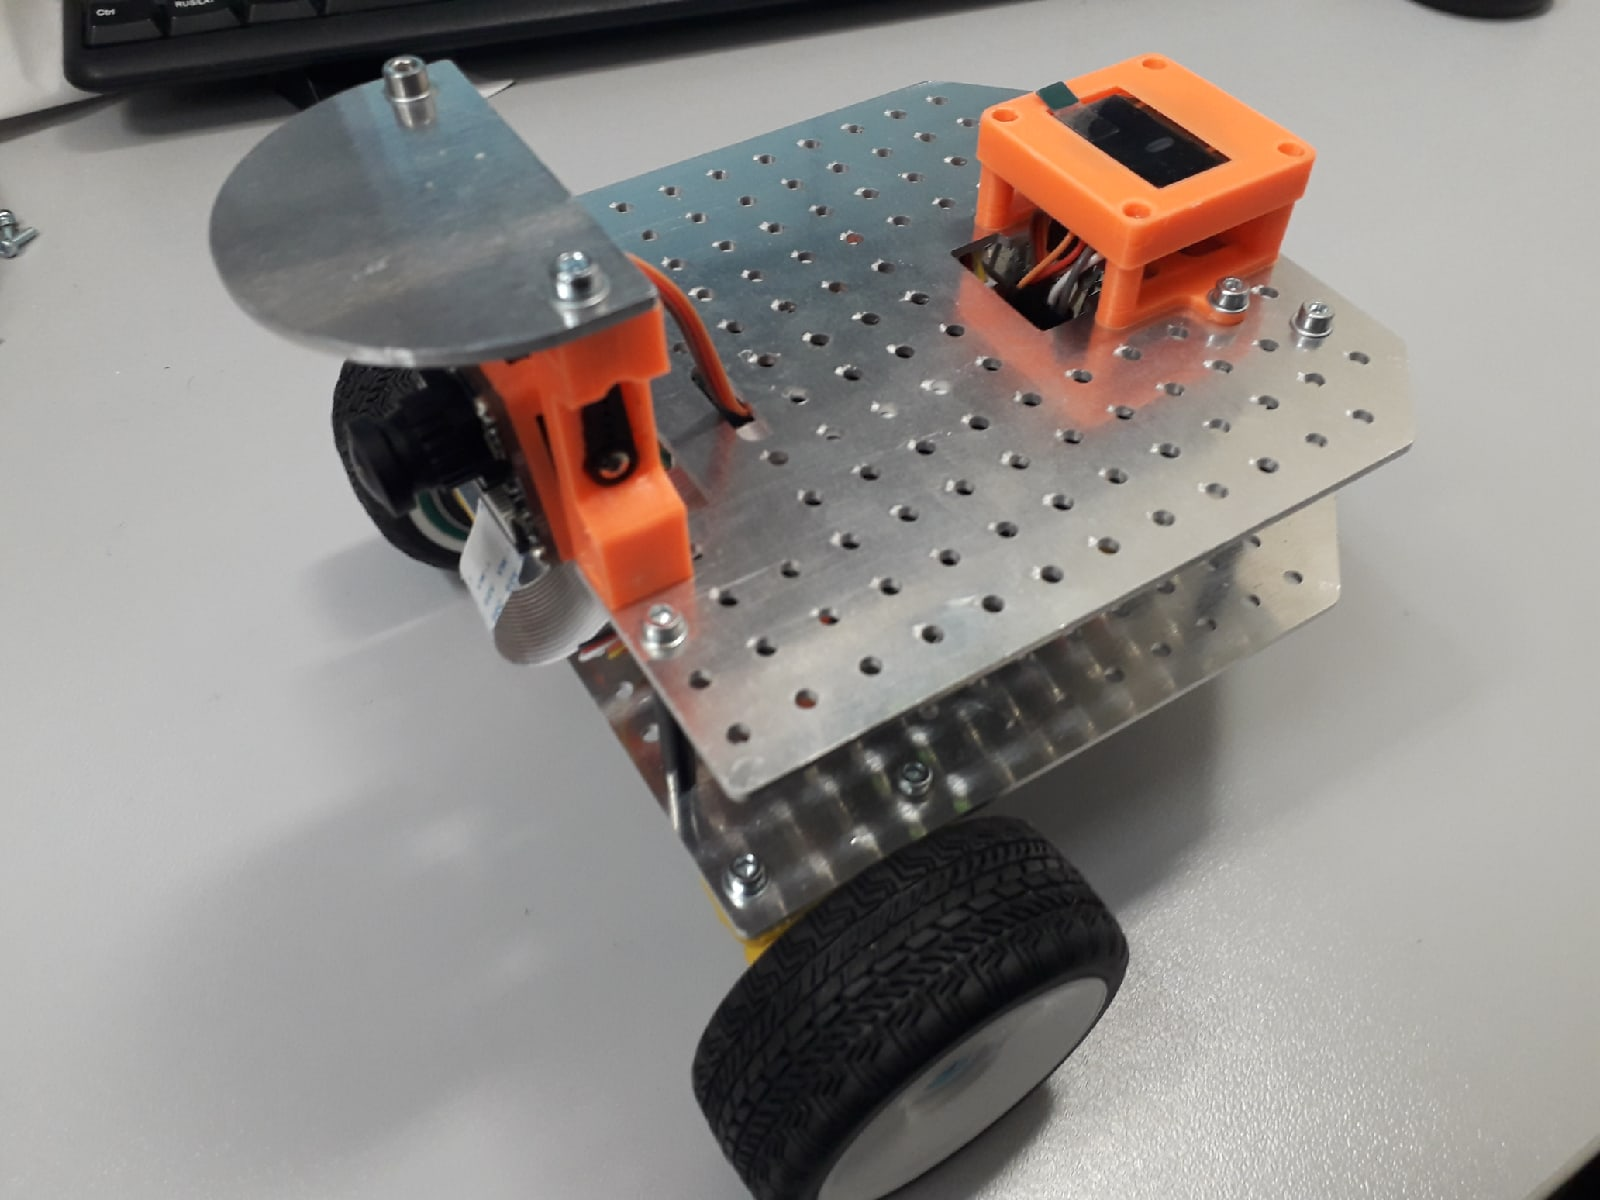
\includegraphics[scale=0.15]{edubot.jpg}
\caption{Edubot}
\label{fig:edubot}
\end{figure}

Структурную схему аппаратной части платформы можно увидеть на рисунке 2. В настоящей версии платформы аппаратная часть сожержит в себе одноплатный компьютер Raspberry pi в качестве базы, к одноплатному компьютеру присоединяется шилд, который обеспечивает взаимодействие с перефирией: моторы, сервоприводы, кнопка, пищалка, датчик тока, а также предоставляет физические разьемы для дисплея и других I2C устройств. Также к одноплатному компьютеру подключена цифровая видеокамера.     

\begin{figure}[h!]
\centering
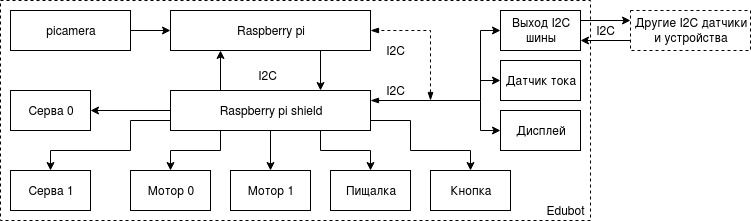
\includegraphics[scale=0.5]{edubot_hardware.jpg}
\caption{Структурная схема аппаратной части платформы Edubot}
\label{fig:edubothardware}
\end{figure}

Изначально, данная платформа, как и другие, выступает в качестве учебной платформы, предназначенной для обучения написания различных программ, поэтому, в дополнение к аппаратному обеспечению, для каждой платформы пишется базовый программный интерфейс на языке программирования python для взаимодействия и управления аппаратной частью (рисунок 3). Данный программный интерфейс представляет собой высокоуровневый интерфейс для взаимодействия с платформой: различные конфигурационные файлы, инструменты, а также низкоуровневый интерфейс, который просто обеспечивает взаимодействие с I2C устройствами (написан также на python). 

\begin{figure}[h!]
\centering
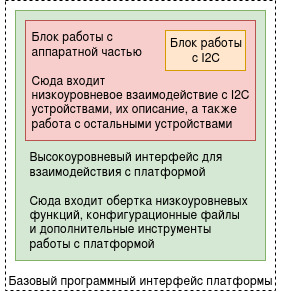
\includegraphics[scale=0.8]{program.jpg}
\caption{Компоненты базового программного интерфейса}
\label{fig:program}
\end{figure}

\section{Проблема взаимодействия}
Предполагается, что на одной платформе одновременно будут работать множество программ, которые будут иметь доступ к аппаратной переферии (в случае Edubot'a это такие программы: автоматическая программа вывода сетевой информации на дисплей, различные серверы, программы управления и т.д.). Если каждая такая программа в себе будет иметь копию базового программного интерфейса или его часть (рисунок 4 (a)), то в этом случае при физическом, аппаратном или другом изменении конфигурации платформы (изменение версии платформы, смена платформы, замена аппаратных компонентов и т.д.) или же просто в случае обновления самого базового программного интерфейса, придется изменять или обновлять каждую копию данной программной части. Для выхода из этого положения, самым простым способом будет использовать одну и ту же копию программного интерфейса, просто импортируя ее из какого-либо одного места (рисунок 4 (b)).

\begin{figure}[h!]
\centering
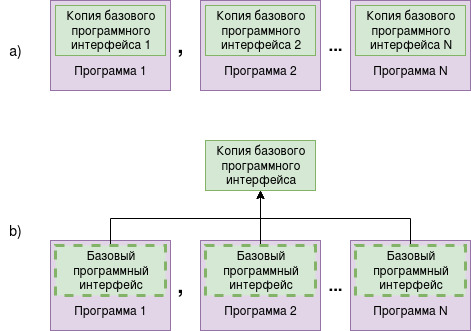
\includegraphics[scale=0.8]{interaction.jpg}
\caption{Взаимодействие программных компонент}
\label{fig:interaction}
\end{figure}

Если рассматривать платформу Edubot в качестве примера, то вышеописанное можно было бы просто реализовать, если низкоуровневый программный интерфейс выпустить в качестве стандартного пакета python, который бы устанавливался вместе со всеми пакетами python и импортировался бы оттуда. Однако, помимо самого низкоуровневого интерфейса присутствуют также различные дополнительные инструменты и конфигурационные файлы, которые варьируются от платформы к платформе, из-за чего придется аналогично рисунку 4 (a) использовать множество их копий в различных программах, что особо ситуацию не изменит.  

По этой причине предлагается попробовать использовать определенную организацию файлов базового интерфейса и других вспомогательных программ для решения проблемы. 

\section{Файловая организация}
Для обеспечения платформонезависимости управляющего кода, а также облегчения создания и деплоя управляющих и иных программ для робототехнических платформ предлагается использовать следующую файловую организацию (рисунок 5).

\begin{figure}[h!]
\centering
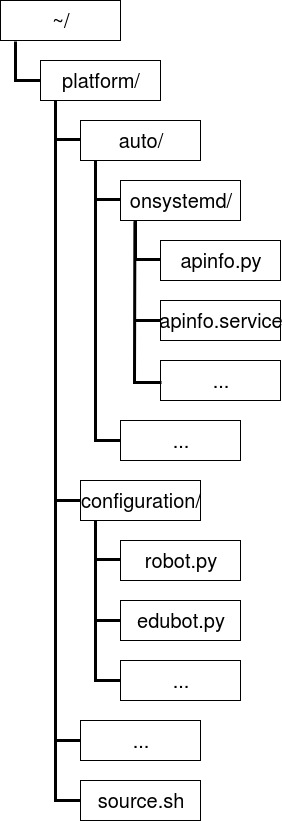
\includegraphics[scale=0.8]{fileorg.jpg}
\caption{Пример предлагаемой файловой организации}
\label{fig:organization}
\end{figure}

В домашней директории располагается директория platform, которая будет содержать все ресурсы и инструменты для работы с роботом. В директории auto располагаются автоматические скрипты и сервисы, которые должны запускаться при включении робота, начале ssh сессии и т.д. В данном примере в auto в поддиректории onsystemd (скрипты, которые должны запускаться при включении робота) лежит скрипт автоматического вывода сетевой информации платформы на дисплей при включении: apinfo.py и его сервис apinfo.service. В поддиректории configuration находится файл конфигурации робота (robot.py) и необходимые для работы ресурсы. Пример конфигурационного файла для платформы Edubot можно увидеть в листинге 1. Файл source.sh автоматизирует некоторую работу: обрабатывает, переносит и запускает сервисы, настраивает другие автоматические программы, производит обновление ПО и т.д. Данная файловая организация пока находится на этапе тестирования и возможно будет дополняться и изменяться. 

\begin{lstlisting}[language=Python, caption=Конфигурационный файл платформы Edubot robot.py]
""" Edubot configuration """
from configuration.edubot import EduBot, MotorMode
import smbus

servoPosLen = 255
middleServoPos = int(servoPosLen / 2)

bus = smbus.SMBus(1)
robot = EduBot(bus)


def move(speed):
    robot.setParrot0(int(-speed))
    robot.setParrot1(int(speed))


def rotate(speed):
    robot.setParrot0(int(speed))
    robot.setParrot1(int(speed))


def setCamera(scale):
    scale = min(max(-1, scale), 1)
    robot.beep()
    robot.setServo0(int(middleServoPos - scale * servoPosLen))


def initializeAll():
    robot.online = True
    robot.start()
    robot.setMotorMode(MotorMode.MOTOR_MODE_PID)
    robot.setParrot0(0)
    robot.setParrot1(0)
    robot.setServo0(int(middleServoPos))
    robot.setServo1(int(middleServoPos))


def release():
    robot.exit()


@property
def online():
    return robot.online


@online.setter
def online(val):
    robot.online = val
\end{lstlisting}

\section{Заключение}
Представленная в документе концепция файловой организации для робототехнических платформ в ближайшее время пройдет проверку на валидность, в случае успеха, данный документ будет расширяться и дальше.  
\end{document}
